The first parameter we measured was the ideal buffer size for random I/O 
on a file. First, let us define what we mean by ``ideal buffer size.'' Since
the time to read data is affected by the amount of data read, we define ideal
buffer size as the size in which we achieve the best throughput (data per second)
with the smallest amount of memory. 

Given the classical formula of Equation~\ref{eq:p1_latency} for the latency 
of a magnetic disk access:

\begin{equation}\label{eq:p1_latency}
Latency = S + R + DataSize/TransferRate + C
\end{equation}

where $S$ = Seek Time, $R$ = Rotational Delay, and $C$ = Controller delay, we 
derive the throughput as $T = \frac{DataSize}{Latency}$. We assume that $S$, $R$, 
and $C$ are roughly constant regardless of size, so we represent them as constant 
$K$ and simplify to Equation~\ref{eq:p1_throughput}:

\begin{equation}\label{eq:p1_throughput}
T = \frac{DataSize}{K + \frac{DataSize}{TransferRate}}
\end{equation}

We expect the throughput to follow the behavior of a rational function
with an asymptote equalling TransferRate as DataSize becomes infinitely large.
Thus, the ideal buffer size for large reads is defined as the minimum DataSize for 
which the throughput is approximately equal to the TransferRate. There is however, 
one more thing to consider. The Linux filesystem requests sizes at a granularity of 
block size, so in actuality $DataSize = \lceil\frac{RequestSize}{BlockSize}\rceil$.
We therefore expect that the best buffer size will be some N*BlockSize since
if RequestSize is less than BlockSize, the disk will fetch more data than
requested and result in excess disk latency. In the virtual machine case, we assume 
that the overhead due to address translation is marginal due to the shadow page 
tables, so we expect the VM throughput to be approximately the same as in the host.

\begin{figure}[b]
\begin{algorithmic}
\FOR {$readSize$ = MIN \TO MAX}
   \STATE clear cache
   \STATE open $file$
   \STATE read 1 byte from the end of the file
   \STATE start\_timer
   \STATE read $readSize$ bytes from $offset$
   \STATE end\_timer and save the result
   \STATE close $file$
   \STATE report times
\ENDFOR
\end{algorithmic}
\caption{Pseudocode for measuring ideal buffer size}
\label{fig:p1code}
\end{figure}


To find both the minimum transfer size of the disk and to find throughput, we used 
the test described by the pseudocode of Figure~\ref{fig:p1code} with some minor 
variations. To find the block size, we used $MIN = 512B$ and $MAX = 64KB$. 
We used $offset=0$ to ensure block aligned reads. We did not clear the cache
between reads in the same run since we wished to measure the minimum number of bytes
fetched from disk. To obtain the throughput of large reads, we used $MIN = 500KB$ and
$MAX = 30MB$. In both we measured the latency to read $readSize$ bytes from disk.
Then we calculated throughput $T$ by dividing readSize by the measured latency. 
However, there were a few aspects we needed to consider in our throughput experiment. 
Since prefetch occurs on sequential read, we avoided the problem of measuring the 
time to retrieve data from the cache instead of disk access time by first reading 
a single byte from the end of the file and then reading from the beginning of the file, 
essentially making the Linux readahead algorithm interpret both reads as random. 
Moreover, we flushed the cache in between each change of the readSize and closed
the file after each read to reset the readahead.


\begin{figure}[t]
	\begin{subfigure}{0.5\textwidth}
	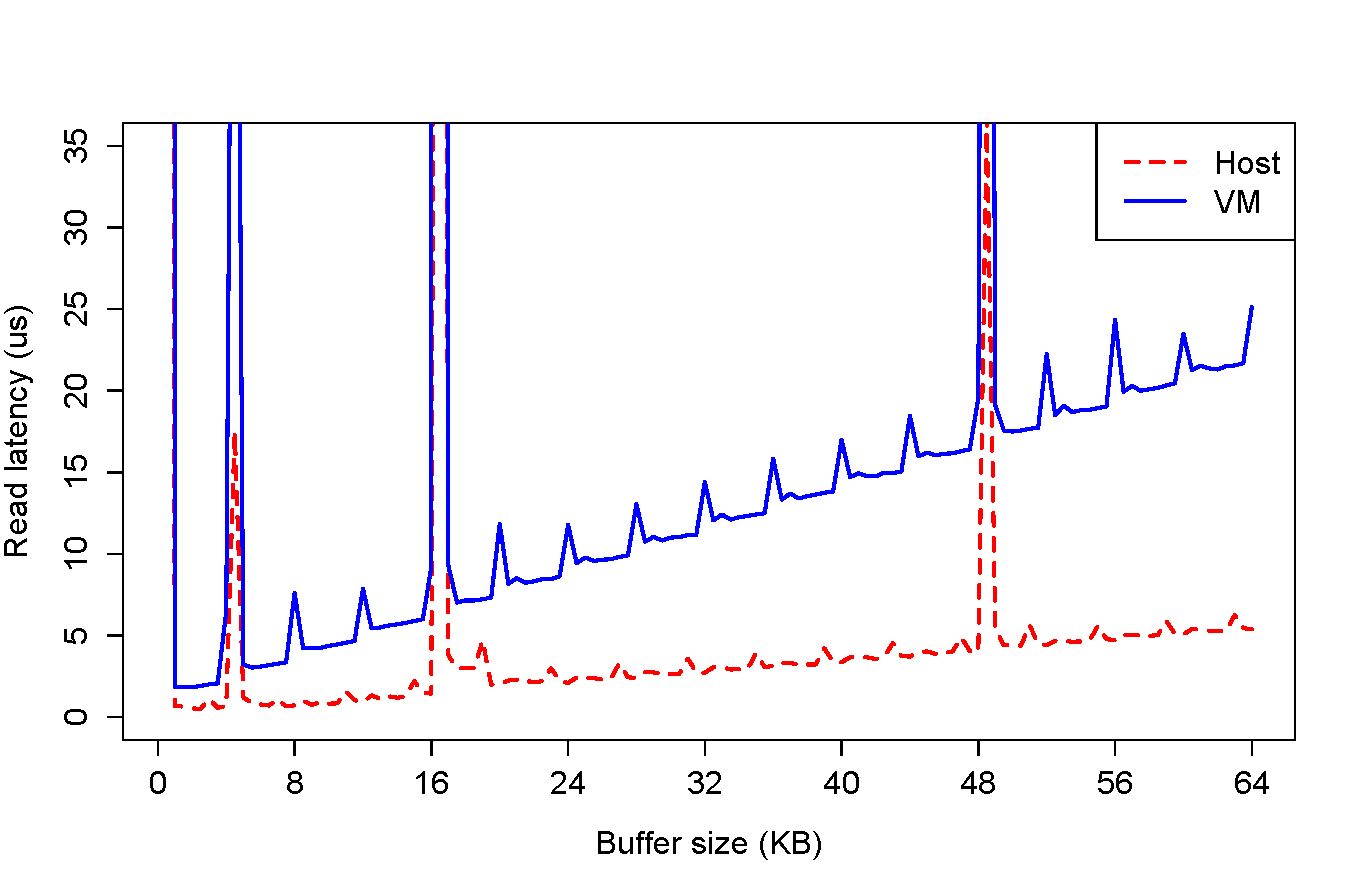
\includegraphics[width=\textwidth]{./figures/p1_new.pdf}
	\caption{Disk latency for small random read sizes}
	\label{fig:p1block}
	\end{subfigure}

	\begin{subfigure}{0.5\textwidth}
	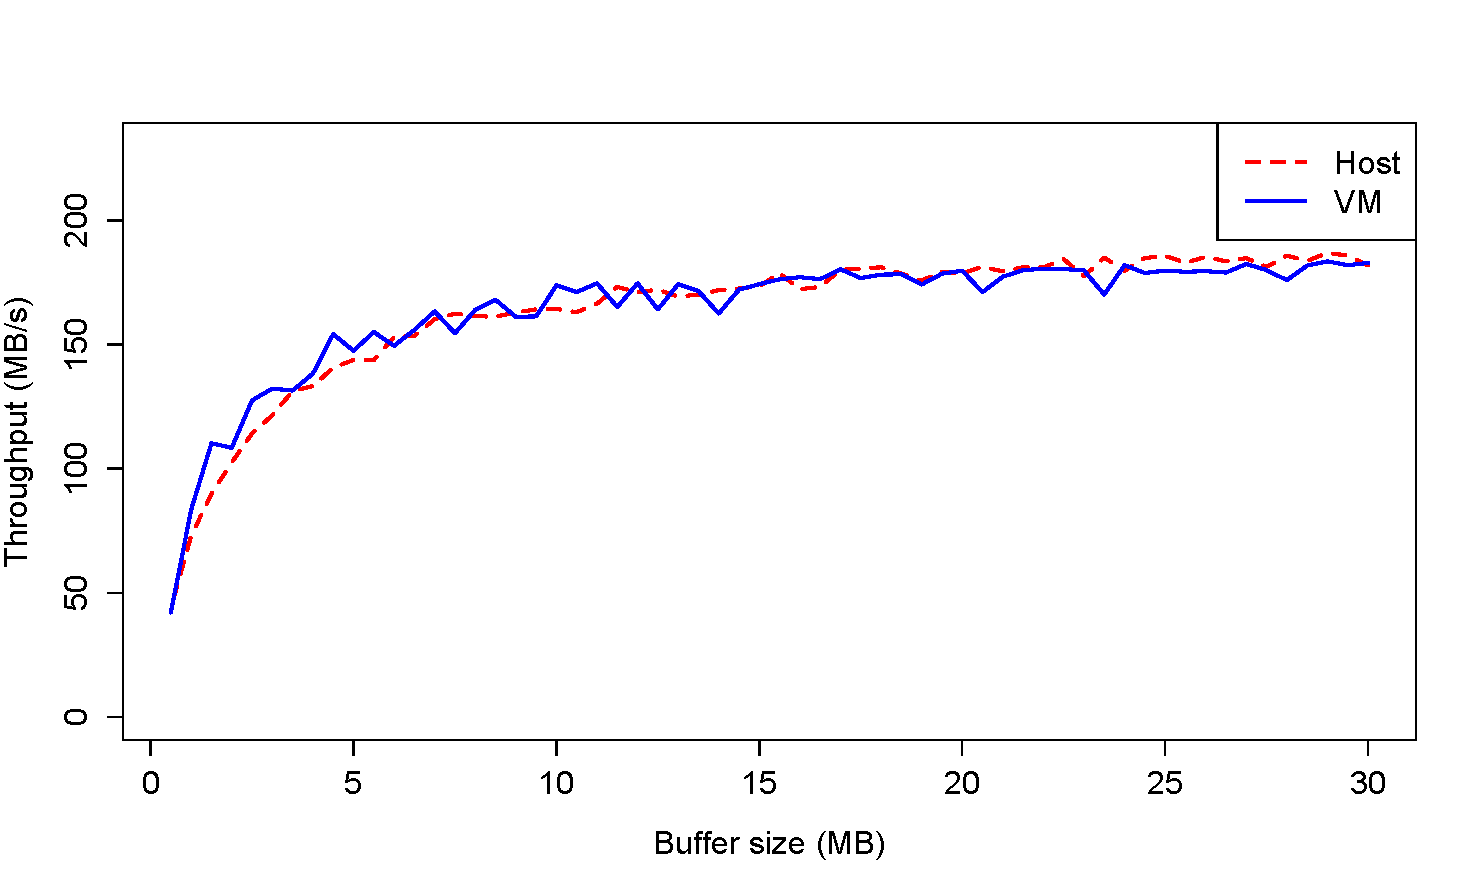
\includegraphics[width=\textwidth]{./figures/p1_old.pdf}
	\caption{Data throughput for large random read sizes}
	\label{fig:p1graph}
	\end{subfigure}
\end{figure}

%% Graphs, Results
We see in Figure~\ref{fig:p1block} that there are peaks in latency every 4KB for 
both the VM and the host. This suggests that the block size is 4KB, the page size
of the system. Notice that the latency diverges linearly between the VM and host,
implying there is some fixed latency per byte experienced by the VM. we get large
spikes at 4KB, 16KB, and 48KB.
In the graph of Figure~\ref{fig:p1graph} we see that throughput of 
both the VM and the host behave
as we expected, with lower read sizes having lower throughput and higher read sizes
having increasing throughput until it approaches an asymptote. We find that the 
maximum throughput is approximately 185MB/s in both cases. Now, we examine a few
points in Figure~\ref{fig:p1graph} to infer the ideal buffer size. We see that when 
the read sizes corresponding throughputs at 86.5\%, 95.0\%, and 98.2\% of the maximum 
throughput are 7MB, 16MB, and 18MB, respectively. We see that at 7MB we just begin to 
approach the plateau and thus the gain in throughput begins to level off.
Note that the jump to 95.0\% maximum throughput requires doubling the read size, 
meaning that the 10\% increase in throughput is at a high memory cost. Similarly, 
changing the read size from 16MB to 18MB gives a 3\% increase in throughput. This 
suggests that 7MB is a good buffer size that maximizes throughput for its size.



